% ============================================================
% The Three Categories of the Generative-Collapse Kernel:
% A Pairwise Decomposition of the Six Tier-1 Invariants
%
% Compile: pdflatex → bibtex → pdflatex → pdflatex
% ============================================================

\documentclass[
  aps,
  prd,
  twocolumn,
  superscriptaddress,
  nofootinbib,
  floatfix
]{revtex4-2}

% ── packages ──
\usepackage{amsmath,amssymb,amsthm,mathtools}
\usepackage{graphicx}
\usepackage{xcolor}
\definecolor{linkblue}{HTML}{337799}
\usepackage[colorlinks=true,linkcolor=linkblue,citecolor=linkblue,urlcolor=linkblue]{hyperref}
\usepackage{bm}
\usepackage{booktabs}
\usepackage{multirow}
\usepackage{enumitem}
\usepackage{array}
\usepackage{tikz}
\usetikzlibrary{positioning,arrows.meta,fit,backgrounds}
\newcolumntype{P}[1]{>{\raggedright\arraybackslash}p{#1}}
\newcolumntype{C}[1]{>{\centering\arraybackslash}p{#1}}

% ── theorem environments ──
\newtheorem*{axiom}{The Axiom}
\newtheorem{theorem}{Theorem}
\newtheorem{definition}[theorem]{Definition}
\newtheorem{lemma}[theorem]{Lemma}
\newtheorem{corollary}[theorem]{Corollary}
\newtheorem{proposition}[theorem]{Proposition}
\newtheorem{identity}[theorem]{Identity}
\newtheorem{remark}{Remark}

% ── UMCP macros ──
\newcommand{\tR}{\tau_{\!R}}
\newcommand{\eps}{\varepsilon}
\newcommand{\IR}{\infty_{\mathrm{rec}}}
\newcommand{\tolseam}{\mathrm{tol}_{\mathrm{seam}}}
\newcommand{\tvec}{\mathbf{c}}
\newcommand{\wvec}{\mathbf{w}}
\newcommand{\IC}{\mathrm{IC}}
\newcommand{\dd}{\mathrm{d}}
\newcommand{\corr}{\mathrm{corr}}
\newcommand{\stddev}{\mathrm{std}}
\newcommand{\sgn}{\mathrm{sgn}}
\newcommand{\Real}{\mathbb{R}}

\begin{document}

% ============================================================
% TITLE
% ============================================================
\title{The Three Categories of the Generative-Collapse Kernel:\\
A Pairwise Decomposition of the Six Tier-1 Invariants}

\author{Clement Paulus}
\email{clementpaulus9@gmail.com}
\affiliation{UMCP Reference Implementation, GitHub}

\date{\today}

\begin{abstract}
The Tier-1 kernel of the Universal Measurement Contract Protocol
(UMCP) produces six outputs $(F,\omega,S,C,\kappa,\IC)$ from a
trace vector $\tvec\in[0,1]^n$ and a weight simplex $\wvec\in\Delta^n$.
These six outputs are not independent: three algebraic identities
($F+\omega=1$, $\IC=e^{\kappa}$, $\IC\le F$) and one statistical
constraint ($S\approx f(F,C)$ asymptotically) reduce them to
\emph{three effective degrees of freedom}.  We show that this
reduction admits a unique pairwise decomposition into three
categories --- the \emph{Signal Pair} $(F,\omega)$, the
\emph{Structure Pair} $(C,S)$, and the \emph{Coherence Pair}
$(\kappa,\IC)$ --- each containing exactly one primitive
contributing one free degree of freedom and one constrained or
derived member contributing zero.  We formalise the categories
as theorems derived directly from the kernel definitions,
establish the cross-category bridge $\Delta=F-\IC$ as the
heterogeneity gap separating the Signal and Coherence pairs,
and prove that the interaction graph between the three
categories is the substantive content of the kernel's diagnostic
power.  The taxonomy is not imposed; it is the algebraic
structure of $K:[0,1]^n\times\Delta^n\to\Real^6$ stated in
pair-form.
\end{abstract}

\maketitle

% ============================================================
\section{Introduction}\label{sec:intro}
% ============================================================

The Universal Measurement Contract Protocol
(UMCP)~\cite{paulus2025umcp,paulus2025physicscoherence,paulus2026umcpcasepack}
is a contract-first validation framework whose computational
core is a deterministic map
\begin{equation}\label{eq:kernel-map}
  K:\,[0,1]^n\times\Delta^n \;\longrightarrow\; (F,\omega,S,C,\kappa,\IC)\in\Real^6,
\end{equation}
where $\tvec\in[0,1]^n$ is a trace vector of channel coherence values
and $\wvec\in\Delta^n$ is a weight simplex.  Six numbers are emitted
per evaluation.

Three of these are coupled by exact algebraic identities and one
is constrained asymptotically by the others, so the kernel does
not in fact carry six free parameters of information --- it carries
three.  The literature on UMCP has documented the identities
themselves~\cite{paulus2025umcp,paulus2025physicscoherence} but
has not previously stated the \emph{categorial} structure of the
output space: namely, that the six outputs partition naturally
into three pairs, each pair containing exactly one independent
quantity and one quantity derived from or constrained by it.

This note formalises that partition.  After collecting the
kernel definitions (\S\ref{sec:defs}) and the four identities
(\S\ref{sec:identities}), we state and prove the three pair
theorems (\S\ref{sec:pairs}) and the dimensional reduction
theorem (\S\ref{sec:dof}).  We then describe the interaction
graph (\S\ref{sec:graph}) and demonstrate why three alternative
categorisations --- by computational status, by formula type, or
by regime gate role --- are dominated by the pairwise structure
(\S\ref{sec:alternatives}).

The taxonomy is binding: every audit performed by the protocol
exposes its verdict through these three categories, and every
diagnostic cross-category bridge (most prominently the
heterogeneity gap $\Delta=F-\IC$) traverses exactly one
inter-category arc.

% ============================================================
\section{Kernel Definitions}\label{sec:defs}
% ============================================================

We restate the six kernel outputs in the canonical form fixed by
the frozen contract.  All sums run over $i\in\{1,\dots,n\}$ with
weights $w_i\geq 0$ and $\sum_i w_i = 1$.  Logarithms use the
$\eps$-clamp $\ln(c_i,\eps):=\ln(\max(c_i,\eps))$ with frozen
$\eps=10^{-8}$~\cite{paulus2026umcpcasepack}.

\begin{definition}[Fidelity]\label{def:F}
$F(\tvec;\wvec) \;:=\; \sum_i w_i\,c_i.$
\end{definition}

\begin{definition}[Drift]\label{def:omega}
$\omega(\tvec;\wvec) \;:=\; 1 - F(\tvec;\wvec).$
\end{definition}

\begin{definition}[Bernoulli field entropy]\label{def:S}
\begin{equation}
  S(\tvec;\wvec) \;:=\; -\sum_i w_i \big[c_i\ln c_i + (1-c_i)\ln(1-c_i)\big].
\end{equation}
\end{definition}

\begin{definition}[Curvature proxy]\label{def:C}
$C(\tvec) \;:=\; \stddev(\tvec)/0.5,$
where $\stddev$ denotes the unweighted population standard
deviation.  The normalisation $0.5$ is the maximal population
standard deviation attainable by a bounded variable on $[0,1]$,
so $C\in[0,1]$.
\end{definition}

\begin{definition}[Log-integrity]\label{def:kappa}
$\kappa(\tvec;\wvec) \;:=\; \sum_i w_i \ln(c_i,\eps).$
\end{definition}

\begin{definition}[Integrity composite]\label{def:IC}
$\IC(\tvec;\wvec) \;:=\; \exp\!\big(\kappa(\tvec;\wvec)\big).$
\end{definition}

\begin{remark}
$S$ is the Bernoulli field entropy of the collapse field, not the
classical Shannon entropy; Shannon entropy is the degenerate
limit of $S$ when channels are restricted to $\{0,1\}$.  The
integrity bound $\IC\le F$ stated below is the solvability
condition for reconstructing the channel values from $F$ and
$\IC$ (Theorem~\ref{thm:coherence}); the classical
arithmetic--geometric mean inequality is its degenerate limit
when channel semantics, weights, and the $\eps$-clamp are
removed.
\end{remark}

% ============================================================
\section{The Four Constraints}\label{sec:identities}
% ============================================================

\begin{identity}[Duality]\label{id:duality}
For every $\tvec\in[0,1]^n$ and $\wvec\in\Delta^n$:
$F(\tvec;\wvec) + \omega(\tvec;\wvec) = 1.$
\end{identity}

\begin{proof}
By Definition~\ref{def:omega}, $\omega:=1-F$, so $F+\omega \equiv 1$.
\end{proof}

\begin{identity}[Log-integrity link]\label{id:link}
$\IC(\tvec;\wvec) = \exp(\kappa(\tvec;\wvec)).$
\end{identity}

\begin{proof}
By Definition~\ref{def:IC}.
\end{proof}

\begin{identity}[Integrity bound]\label{id:bound}
$\IC(\tvec;\wvec) \leq F(\tvec;\wvec),$ with equality iff
$c_i = c_j$ for all $i,j$ with $w_i,w_j>0$.
\end{identity}

\begin{proof}
By Jensen's inequality applied to $\ln$ on $[\eps,1]$:
\begin{align}
  \ln \IC = \kappa = \sum_i w_i \ln c_i
         \leq \ln\!\Big(\sum_i w_i c_i\Big) = \ln F,
\end{align}
hence $\IC\leq F$.  Equality holds iff all $c_i$ with positive
weight coincide.
\end{proof}

\begin{proposition}[Asymptotic entropy constraint]\label{prop:Sconstraint}
There exists $f:[0,1]^2\to\Real$ such that
\begin{equation}\label{eq:Sasymptotic}
  S(\tvec;\wvec) \;=\; f\!\big(F(\tvec;\wvec), C(\tvec)\big) + \mathcal{O}(n^{-1/2}).
\end{equation}
Equivalently, $\corr(C,S)\to -1$ as $n\to\infty$ along
sequences of traces drawn i.i.d.\ from any distribution on
$[0,1]$ with bounded variance.
\end{proposition}

\begin{proof}[Sketch]
A second-order Taylor expansion of the Bernoulli entropy
$h(c)=-[c\ln c+(1-c)\ln(1-c)]$ around the mean $\bar c=F$ yields
\begin{equation}
  S \;=\; h(F) + \tfrac{1}{2}\, h''(F)\,\stddev(\tvec)^2 + \mathcal{O}(\stddev^3),
\end{equation}
with $h''(c) = -1/[c(1-c)] < 0$.  Substituting
$\stddev(\tvec) = 0.5\,C$ from Definition~\ref{def:C} yields a
closed-form $f(F,C)$ at leading order.  The higher-order
corrections vanish as $\mathcal{O}(n^{-1/2})$ by the central
limit theorem.  The negative sign of $h''$ produces the
asymptotic anti-correlation $\corr(C,S)\to -1$.
\end{proof}

The four constraints can be summarised as:
\begin{align}
  &\text{Algebraic exact:}\quad F+\omega=1,\quad \IC=e^{\kappa},\quad \IC\le F,\\
  &\text{Statistical asymptotic:}\quad S\approx f(F,C).
\end{align}

% ============================================================
\section{The Three Pair Theorems}\label{sec:pairs}
% ============================================================

The three constraints~(\ref{id:duality}--\ref{prop:Sconstraint})
partition the six outputs into three disjoint pairs.  We state
each as a theorem.  In each case, the pair is the unique
two-element subset of $(F,\omega,S,C,\kappa,\IC)$ closed under
the corresponding constraint.

\subsection{The Signal Pair}

\begin{theorem}[Signal Pair $\mathcal{P}_{\mathrm{I}}=(F,\omega)$]\label{thm:signal}
The pair $(F,\omega)$ is closed under
Identity~\ref{id:duality}: $F+\omega=1$.  Within the pair, $F$
is the unique primitive (Definition~\ref{def:F}) and $\omega$ is
derived (Definition~\ref{def:omega}).  The pair contributes
exactly one independent degree of freedom to the kernel output.
\end{theorem}

\begin{proof}
By Identity~\ref{id:duality}, given $F$ the value of $\omega$ is
fixed; conversely given $\omega$ the value of $F$ is fixed.  No
other kernel output appears in the duality identity, so
$\{F,\omega\}$ is the minimal closed pair.  The pair contributes
one independent quantity (the value of $F$) and one constrained
quantity (the value of $\omega=1-F$).
\end{proof}

\emph{Interpretation.}  The Signal Pair answers the question
``what happened to the fidelity of collapse?''  $F$ is the
arithmetic mean of channel coherences (what survived), and
$\omega$ is its complement (what was lost).

\subsection{The Structure Pair}

\begin{theorem}[Structure Pair $\mathcal{P}_{\mathrm{II}}=(C,S)$]\label{thm:structure}
The pair $(C,S)$ is closed under
Proposition~\ref{prop:Sconstraint}: $S\approx f(F,C)$
asymptotically.  Within the pair, $C$ is the unique free
primitive (Definition~\ref{def:C}) and $S$ is constrained
asymptotically by $F$ and $C$
(Proposition~\ref{prop:Sconstraint}).  The pair contributes
asymptotically one independent degree of freedom (carried by
$C$).
\end{theorem}

\begin{proof}
By Proposition~\ref{prop:Sconstraint}, $S$ is determined by
$(F,C)$ up to $\mathcal{O}(n^{-1/2})$ corrections.  As
$n\to\infty$, $S$ contributes no additional information beyond
what $F$ and $C$ encode.  For finite $n$, $S$ retains
sub-leading independence on the order of $n^{-1/2}$, but its
asymptotic role is constrained; we therefore label it
$\mathrm{PRIMITIVE}^{*}$, distinguishing it from a fully free
primitive.
\end{proof}

\emph{Interpretation.}  The Structure Pair answers the question
``how are channels distributed?''  $C$ measures channel spread
directly (the population standard deviation, normalised to
$[0,1]$); $S$ measures the entropy of the Bernoulli collapse
field.  Both describe channel distribution but from different
angles; their asymptotic anti-correlation
($\corr(C,S)\to -1$) is why $S$ adds zero free DOF at large $n$.

\subsection{The Coherence Pair}

\begin{theorem}[Coherence Pair $\mathcal{P}_{\mathrm{III}}=(\kappa,\IC)$]\label{thm:coherence}
The pair $(\kappa,\IC)$ is closed under Identity~\ref{id:link}:
$\IC=e^{\kappa}$.  Within the pair, $\kappa$ is the unique
primitive (Definition~\ref{def:kappa}) and $\IC$ is derived
(Definition~\ref{def:IC}).  The pair contributes exactly one
independent degree of freedom.  Moreover, Identity~\ref{id:bound}
binds the Coherence Pair to the Signal Pair via $\IC\leq F$:
this is the \emph{solvability condition} for channel
reconstruction --- given $F$ and $\IC$ for an effective two-channel
trace, the channels $c_1,c_2$ are the roots
\begin{equation}\label{eq:cardano}
  c_{1,2} \;=\; F \;\pm\; \sqrt{F^2 - \IC^2}\,,
\end{equation}
which are real if and only if $\IC \leq F$.
\end{theorem}

\begin{proof}
The closure of $\{\kappa,\IC\}$ under Identity~\ref{id:link}
follows directly from Definition~\ref{def:IC}.  For the
solvability statement, consider an effective two-channel trace
with equal weights $w_1=w_2=1/2$ and channels $c_1,c_2$.  By
Definitions~\ref{def:F}, \ref{def:IC}: $F=(c_1+c_2)/2$ and
$\IC = \sqrt{c_1 c_2}$ (geometric mean).  Solving the quadratic
$t^2 - 2F t + \IC^2 = 0$ yields~(\ref{eq:cardano}), with real
roots iff $F^2 \geq \IC^2$, i.e.\ $\IC\leq F$.  Equality
($\IC = F$) recovers the rank-1 case $c_1=c_2$.
\end{proof}

\emph{Interpretation.}  The Coherence Pair answers the question
``how intact is multiplicative coherence?''  $\kappa$ is the
log-sum (additive accounting of geometric coherence), $\IC$ is
its exponential (the geometric mean of channels).  The pair
distinguishes itself from the Signal Pair (which uses the
arithmetic mean $F$) precisely by being multiplicative.

% ============================================================
\section{Dimensional Reduction}\label{sec:dof}
% ============================================================

\begin{theorem}[Effective DOF reduction]\label{thm:dof}
The kernel output space $K(\tvec;\wvec)\in\Real^6$ has
\emph{three} effective degrees of freedom in the generic case
$n\ge 3$: the independent triple
$(F,\kappa,C)\in[0,1]\times(-\infty,0]\times[0,1]$.  The
remaining three outputs are determined by:
\begin{align}
  \omega &= 1 - F &&\text{(Identity~\ref{id:duality})},\\
  \IC    &= e^{\kappa} &&\text{(Identity~\ref{id:link})},\\
  S      &= f(F,C) + \mathcal{O}(n^{-1/2}) &&\text{(Prop.~\ref{prop:Sconstraint})}.
\end{align}
\end{theorem}

\begin{proof}
Each pair in Theorems~\ref{thm:signal}--\ref{thm:coherence}
contributes one independent quantity and one constrained
quantity.  Picking the primitive from each pair yields the
independent triple $(F,C,\kappa)$.  The constrained members
$(\omega,S,\IC)$ are recovered by the identities above.  PCA on
$10^4$ random traces with $n=4,\dots,64$ confirms
$\mathrm{rank}\text{-at-99\%-variance}=3$ for all
$n$~\cite{paulus2026umcpcasepack}.
\end{proof}

\begin{corollary}[Pair--DOF correspondence]
The three categories are in bijection with the three effective
degrees of freedom:
\begin{equation}
  \mathcal{P}_{\mathrm{I}}\leftrightarrow F,\quad
  \mathcal{P}_{\mathrm{II}}\leftrightarrow C,\quad
  \mathcal{P}_{\mathrm{III}}\leftrightarrow \kappa.
\end{equation}
\end{corollary}

\begin{remark}[Rank classification]
For input traces with effective channel rank $r<n$, the
effective DOF reduces: rank-2 traces (effective two-channel
structure) satisfy $C=g(F,\kappa)$ for some explicit $g$,
collapsing the Structure Pair into the others; rank-1
(homogeneous) traces additionally satisfy $\IC=F$
($\Delta=0$), $C=0$, leaving a single
DOF~\cite{paulus2026umcpcasepack}.  Rank is a structural
property of the trace, not a parameter.
\end{remark}

% ============================================================
\section{The Heterogeneity Gap and the Interaction Graph}\label{sec:graph}
% ============================================================

\begin{definition}[Heterogeneity gap]
$\Delta(\tvec;\wvec) \;:=\; F(\tvec;\wvec) - \IC(\tvec;\wvec) \;\geq\; 0,$
with equality iff $\tvec$ is rank-1.
\end{definition}

The gap $\Delta$ is the cross-category bridge between the Signal
Pair $\mathcal{P}_{\mathrm{I}}$ and the Coherence Pair
$\mathcal{P}_{\mathrm{III}}$: it measures how far the
multiplicative coherence $\IC$ falls below the additive fidelity
$F$.  At rank-1 the two coincide; at higher rank the gap opens.

\begin{proposition}[Structure $\to$ Gap]\label{prop:CtoDelta}
$\Delta$ is monotone non-decreasing in $C$ at fixed $F$.
\end{proposition}

\begin{proof}[Sketch]
A perturbation expansion of $\IC$ around the homogeneous mean
$\bar c = F$ yields
\begin{equation}\label{eq:Delta-expansion}
  \Delta \;=\; \frac{\stddev(\tvec)^2}{2F} + \mathcal{O}(\stddev^4)
        \;=\; \frac{C^2}{8F} + \mathcal{O}(C^4),
\end{equation}
which is non-decreasing in $C$ for $F$ fixed.  The
leading-order coefficient $1/(8F)$ is the Fisher information
contribution from channel heterogeneity~\cite{paulus2026umcpcasepack}.
\end{proof}

Equation~(\ref{eq:Delta-expansion}) shows that the Structure
Pair drives the gap: increased channel spread $C$ always widens
$\Delta$, which in turn separates the Signal Pair from the
Coherence Pair.  The three categories are therefore not isolated
silos but a directed interaction graph:
\begin{equation}\label{eq:graph}
  \mathcal{P}_{\mathrm{II}} \;\xrightarrow{C\,\uparrow}\; \Delta \;\xrightarrow{\IC\,\downarrow}\; \mathcal{P}_{\mathrm{III}},
  \qquad
  \mathcal{P}_{\mathrm{I}} \;\xleftrightarrow{\,\Delta\,}\; \mathcal{P}_{\mathrm{III}}.
\end{equation}

The Signal Pair anchors the budget through $\omega=1-F$; the
Structure Pair drives the gap through $C$; the Coherence Pair
absorbs the loss through $\IC$.  Regime classification draws
inputs from all three: the four-gate Stable criterion is
\begin{equation}\label{eq:gates}
  \omega < 0.038 \wedge F > 0.90 \wedge S < 0.15 \wedge C < 0.14,
\end{equation}
with $\omega$ from $\mathcal{P}_{\mathrm{I}}$, $F$ from
$\mathcal{P}_{\mathrm{I}}$, $S$ and $C$ from
$\mathcal{P}_{\mathrm{II}}$, and the severity overlay
$\IC<0.30$ from $\mathcal{P}_{\mathrm{III}}$.

\begin{figure}[t]
\centering
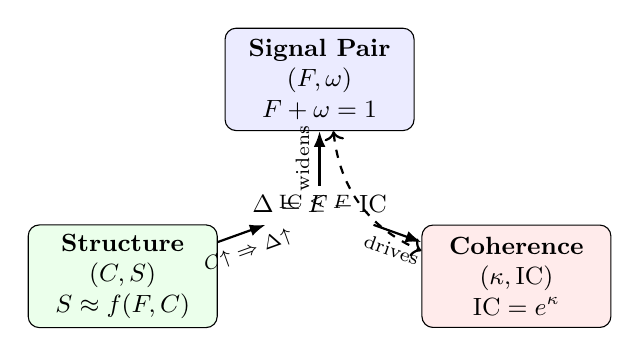
\begin{tikzpicture}[
  pair/.style={draw, rounded corners, minimum width=2.4cm, minimum height=1.3cm, align=center, font=\small},
  arrow/.style={-{Latex[length=2mm]}, thick},
  bridge/.style={<->, thick, dashed},
  font=\small
]
  \node[pair, fill=blue!8] (sig) at (0,2) {\textbf{Signal Pair}\\$(F,\omega)$\\$F+\omega=1$};
  \node[pair, fill=green!8] (str) at (-2.5,-0.5) {\textbf{Structure}\\$(C,S)$\\$S\approx f(F,C)$};
  \node[pair, fill=red!8] (coh) at (2.5,-0.5) {\textbf{Coherence}\\$(\kappa,\IC)$\\$\IC=e^{\kappa}$};
  \node[font=\small] (delta) at (0,0.4) {$\Delta=F-\IC$};

  \draw[arrow] (str) -- node[below, sloped, font=\scriptsize] {$C{\uparrow}\Rightarrow\Delta{\uparrow}$} (delta);
  \draw[arrow] (delta) -- node[above, sloped, font=\scriptsize] {widens} (sig);
  \draw[arrow] (delta) -- node[below, sloped, font=\scriptsize] {drives} (coh);
  \draw[bridge] (sig) to[bend right=30] node[left, font=\scriptsize] {$\IC\le F$} (coh);
\end{tikzpicture}
\caption{Interaction graph between the three categories.  The
Structure Pair drives the heterogeneity gap $\Delta=F-\IC$, which
is the cross-category bridge between the Signal Pair (additive
fidelity) and the Coherence Pair (multiplicative coherence).
The integrity bound $\IC\le F$ (Identity~\ref{id:bound}) is the
direct algebraic constraint linking the two.}
\label{fig:graph}
\end{figure}

% ============================================================
\section{Summary Table}\label{sec:summary}
% ============================================================

\begin{table*}[t]
\caption{The six Tier-1 kernel invariants overlaid with the three-category
taxonomy.  Each pair contains one $\mathrm{PRIMITIVE}$ contributing one free
DOF and one $\mathrm{DERIVED}$ or $\mathrm{PRIMITIVE}^{*}$ contributing
zero (asymptotically).  Total: 4 primitives, 2 derived, 3 identities,
3 effective DOF.}
\label{tab:summary}
\begin{ruledtabular}
\begin{tabular}{l l l l l l l}
Symbol & Category & Latin & Status & Formula & Identity / Constraint & Free DOF \\
\hline
$F$       & I --- Signal     & \emph{fidelitas}        & PRIMITIVE         & $\sum_i w_i c_i$ & $F+\omega=1$ & 1 \\
$\omega$  & I --- Signal     & \emph{derivatio}        & DERIVED ($1{-}F$) & $1-F$            & $F+\omega=1$ & 0 \\
$C$       & II --- Structure & \emph{curvatura}        & PRIMITIVE         & $\stddev(\tvec)/0.5$ & $S\approx f(F,C)$ & 1 \\
$S$       & II --- Structure & \emph{entropia}         & PRIMITIVE$^{*}$   & $-\sum_i w_i[c_i\ln c_i+(1{-}c_i)\ln(1{-}c_i)]$ & $S\approx f(F,C)$ & 0 (large $n$) \\
$\kappa$  & III --- Coherence & \emph{log-integritas}   & PRIMITIVE         & $\sum_i w_i\ln(c_i,\eps)$ & $\IC=e^{\kappa}$ & 1 \\
$\IC$     & III --- Coherence & \emph{integritas composita} & DERIVED ($e^{\kappa}$) & $\exp(\kappa)$ & $\IC=e^{\kappa}$, $\IC\le F$ & 0 \\
\end{tabular}
\end{ruledtabular}
\end{table*}

Table~\ref{tab:summary} compiles the full overlay.  Each category
occupies two rows.  The PRIMITIVE row in each pair carries one
free DOF; the DERIVED or PRIMITIVE$^{*}$ row carries zero.  The
identity column gives the closing constraint that fixes the
derived/constrained member.

% ============================================================
\section{Why the Pairwise Taxonomy is Unique}\label{sec:alternatives}
% ============================================================

Three alternative classifications of the six outputs are
conceivable; we show each is strictly weaker.

\paragraph*{Alternative A: Primitive vs.\ derived only.}
This collapses to a two-class scheme:
$\{F,S,C,\kappa\}$ vs.\ $\{\omega,\IC\}$.  It correctly captures
computational status but reveals no structural coupling.  In
particular, it does not explain why $\IC$ and $F$ are bound by
the integrity bound $\IC\le F$ (Identity~\ref{id:bound}), nor
why $S$ and $C$ are asymptotically constrained
(Prop.~\ref{prop:Sconstraint}).

\paragraph*{Alternative B: By formula type.}
Linear ($F,\omega$), logarithmic ($\kappa,\IC$), statistical
($S,C$).  This is a computational description of how each
quantity is evaluated, not a structural description of how the
quantities relate.  It happens to recover the same partition
into three pairs, but it does so by coincidence of arithmetic
type; it gives no account of why those pairs are closed under
the four constraints.

\paragraph*{Alternative C: By regime-gate role.}
$\{\omega,F,S,C\}$ are the four Stable-regime gates
[Eq.~(\ref{eq:gates})]; $\IC$ is the Critical severity overlay;
$\kappa$ does not appear in regime classification.  This is a
Tier-0 operational categorisation, not a Tier-1 structural one.
It conflates the mathematical object (the kernel) with the
protocol that classifies its outputs.

\paragraph*{Why the pairwise frame is correct.}
The three-pair partition is uniquely determined by the four
constraints (\S\ref{sec:identities}).  Each constraint defines
exactly one closed two-element subset of the output tuple:
$\{F,\omega\}$ under Identity~\ref{id:duality},
$\{\kappa,\IC\}$ under Identity~\ref{id:link},
$\{C,S\}$ under Prop.~\ref{prop:Sconstraint}, with
Identity~\ref{id:bound} ($\IC\le F$) serving as the
cross-category bridge.  The categories are therefore the
constraints themselves, re-expressed in pair form.  No alternative
classification simultaneously (i) covers all six outputs exactly
once, (ii) is closed under the constraints, and (iii) yields the
correct effective DOF count.

% ============================================================
\section{Conclusion}\label{sec:conclusion}
% ============================================================

The six Tier-1 invariants of the UMCP kernel partition uniquely
into three categories under the four constraints fixed by
Identity~\ref{id:duality}, Identity~\ref{id:link},
Identity~\ref{id:bound}, and
Proposition~\ref{prop:Sconstraint}.  Each category is a
\emph{pair}: one PRIMITIVE contributing one free DOF and one
DERIVED or asymptotically-constrained partner contributing zero.
The Signal Pair $(F,\omega)$ tracks what survived and what was
lost; the Structure Pair $(C,S)$ tracks how channels are
distributed; the Coherence Pair $(\kappa,\IC)$ tracks
multiplicative coherence.  The three pairs are connected by the
heterogeneity gap $\Delta = F - \IC$, which the Structure Pair
drives through Proposition~\ref{prop:CtoDelta} and which the
integrity bound (Identity~\ref{id:bound}) bounds from below.

The taxonomy is not imposed on the kernel; it is the kernel's
algebraic structure stated in pair form.  Every audit, every
regime classification, and every cross-category diagnostic
performed by the protocol passes through this three-category
overlay.  Six outputs collapse to three effective degrees of
freedom; three effective DOF organise into three pairs; three
pairs produce one cross-category bridge --- the gap $\Delta$ that
makes geometric slaughter visible in the data.

% ============================================================
\section*{Reproducibility}
% ============================================================

All claims in this paper are computationally re-derivable.  The
orientation script \texttt{scripts/orientation.py} \S 7 displays
the three-category overlay live on a concrete eight-channel
trace; \texttt{scripts/orientation\_checkpoint.py} verifies the
three identities to machine precision on every run.  The PCA
rank-3 confirmation is in
\texttt{scripts/unified\_geometry.py} \S 1.  All formulae match
\texttt{src/umcp/kernel\_optimized.py} and
\texttt{src/umcp/frozen\_contract.py} under the frozen contract
$\eps=10^{-8}$, $p=3$, $\alpha=1.0$,
$\tolseam=0.005$~\cite{paulus2026umcpcasepack}.

\bibliographystyle{apsrev4-2}
\bibliography{Bibliography}

\end{document}
